\documentclass[10pt,twocolumn,letterpaper]{article}

\usepackage{cvpr}
\usepackage{times}
\usepackage{epsfig}
\usepackage{graphicx}
\usepackage{amsmath}
\usepackage{amssymb}
\usepackage{booktabs}
\usepackage{microtype}
% From https://ctan.org/pkg/matlab-prettifier
\usepackage[numbered,framed]{matlab-prettifier}
\newcommand{\vect}[1]{\boldsymbol{\mathbf{#1}}}
\DeclareMathOperator*{\argmax}{arg\,max}
\DeclareMathOperator*{\argmin}{arg\,min}
\frenchspacing

% Include other packages here, before hyperref.

% If you comment hyperref and then uncomment it, you should delete
% egpaper.aux before re-running latex.  (Or just hit 'q' on the first latex
% run, let it finish, and you should be clear).
\usepackage[pagebackref=true,breaklinks=true,letterpaper=true,colorlinks,bookmarks=false]{hyperref}

\cvprfinalcopy % *** Uncomment this line for the final submission

\def\cvprPaperID{****} % *** Enter the CVPR Paper ID here
\def\httilde{\mbox{\tt\raisebox{-.5ex}{\symbol{126}}}}

% Pages are numbered in submission mode, and unnumbered in camera-ready
\ifcvprfinal\pagestyle{empty}\fi
\begin{document}

%%%%%%%%% TITLE
\title{CSCI 1430 Final Project Report:\\Your project title}

\author{\emph{Team name}: First member, second member, third member, fourth member.\\
Brown University\\
19th December 2017
}

\maketitle
%\thispagestyle{empty}

%%%%%%%%% ABSTRACT
% [1430: James] We'll ignore the abstract for now.
\begin{abstract}
In this project, the application of variational inference for visual domain adaptation problem is explored. We leverage the power of deep neural network to learn features from data set, and construct a family of distribution for domain adaptation. We will first introduce the visual domain adaptation problem. Secondly, we will recap the basics of variational inference technique. Thirdly, this report will explore the use of natural gradient descent to improve variational inference.
\end{abstract}

%%%%%%%%% BODY TEXT
\section{Domain Adaptation}

Domain Adaptation is the task of adapting a model trained in one domain, called the \textit{source} domain, to another domain, called the \textit{target} domain. The source domain data is usually fully labeled but we only have access to data from target domain with no label (hence unsupervised).
Although there are several different setup of the problem, we only focus here on the unsupervised domain adaptation with classification as objective.

Formally we have, a joint space of inputs and class labels, \(\mathcal{X} \times \mathcal{Y}\) where \(\mathcal{Y} = \{1,\dots,K\}\). 
Suppose we have two domains on this space, the \textbf{source (S)} and the \textbf{target (T)}, defined by unknown distributions 
\(p_S(\vect{x}, y)\) 
and 
\(p_T(\vect{x},y)\).
We are given source-domain training examples with labels \(\mathcal{D}_S = \{\vect{x}_i^S, y_i\}_{i=1}^{N_S}\) and target data \(\mathcal{D}_T = \{\vect{x}_I^T\}_{i=1}^{N_T}\) without labels.
Assuming a \textbf{shared set of class labels} between the two domains. The goal is to assign the correct class labels to target data points.

This problem is tackled in a shared latent space framework, where we seek to learn an embedding function \(G: \mathcal{X} \to \mathcal{Z}\) and a classifier \(h: \mathcal{Z} \to \mathcal{Y}\).
The functions \(G(\cdot)\) and \(h(\cdot)\) are shared across both domain and will be used to classify samples from target domain, i.e. \(y = h(G(\vect{x}))\), where \(\vect{x} \sim p_T\).

\subsection{Gaussian Process Classifier}
We model \(K\) underlying latent functions \(\vect{f} = \{f_i\}_{i=1}^{K}\) on shared space, \(\mathcal{Z}\), as \(K\)-class Gaussian Process (GP) classifier, 
    \begin{equation} \label{eq:prior}
        p(\vect{f}) = \prod_{i=1}^{K}P(f_i), \, f_i \sim \mathcal{GP}\left(0, \kappa_j(\cdot,\cdot)\right)
    \end{equation}
where \(\kappa_j(\cdot,\cdot)\) is the covariance function of the GP. Using the likelihood model,
    \begin{equation} \label{eq:likfunc}
        P(y=i | \vect{f}(\vect{z})) = \frac{e^{f_i(\vect{z})}}{\sum_{j=1}^{K}e^{f_j(\vect{z})}}, \, i = 1,\dots,K
    \end{equation}
we get that \(\mathcal{D}_{_{S}}\) induces a posterior distribution on \(\vect{f}\),
    \begin{equation} \label{eq:targetpost}
        p(\vect{f}|\mathcal{D}_{_{S}}) \propto p(\vect{f}) \cdot \prod_{i=1}^{N_s} P(y_i^{S} | \vect{f}(\vect{z}_i^{S}))
    \end{equation}

\subsection{Deep Kernel Trick}
Up to this point, the \(\kappa_j\)'s in (\ref{eq:prior}) is only computable by limited choice of \(\kappa_j\). 
We use the deep kernel trick to elevate this problem but modeling the \(\kappa_j\) with a nonlinear feature map \(\phi: \mathcal{Z} \to \mathbb{R}^d\) defined as an inner product in the feature space.

Assuming \(\vect{w}_i \sim \mathcal{N}(\vect{0}, \vect{I})\), then the \(\mathcal{H}\) prior (\ref{eq:targetpost}) becomes,
    \begin{equation}
        p(\vect{W}|\mathcal{D}_{_{S}}) \propto \prod_{i=1}^{K}\mathcal{N}(\vect{w}_i ; \vect{0}, \vect{I}) \cdot \prod_{i=1}^{N_s} P(y_i^{S} | \vect{W \phi}(\vect{z}_i^{S}))
    \end{equation}
    
Note that \(p(\vect{W}|\mathcal{D}_{_{S}})\) is still intractable, and the next section will explain a technique to approximate it.

\section{Variational Inference}
Variation Bayesian methods is a family of techniques for approximating intractable (posterior) distribution arising in Bayesian inference. 
Given an intractable posterior distribution \(p(\vect{z}|\vect{x})\), where \(\vect{z}\) is latent variable and \(\vect{x}\) is some data.
We approximate \(p(\vect{z}|\vect{x})\) with a variational distribution \(q(\vect{z})\). The variational distribution is chosen to be simpler (tractable and factorizable) than the posterior. 

We choose \(q(\vect{z})\) to be,
\[
q(\vect{z}) = \prod_{i=1}^{K} \mathcal{N}(\vect{w}_i ; \vect{m}_i, \vect{S}_i)
\]
For the approximation we look at the KL-divergence,
\begin{align*}
    D_{_{KL}}(q(\vect{z}) || p(\vect{z} | \vect{x})) &= \mathbb{E}_{q(\vect{z})} \left[ \log \frac{q(\vect{z})}{p(\vect{z} | \vect{x})} \right] \\
    &= \mathbb{E}_{q(\vect{z})} \log q(\vect{z}) - \log p(\vect{z} | \vect{x}) \\
    &= \mathbb{E}_{q(\vect{z})} \log q(\vect{z}) - \log \frac{p(\vect{x}, \vect{z})}{p(\vect{x})} \\
    &= \mathbb{E}_{q(\vect{z})} \log q(\vect{z}) - \log p(\vect{x}|\vect{z}) p(\vect{z}) \\
    &+ \log p(\vect{x})\\
    &= \mathbb{E}_{q(\vect{z})} \log \frac{q(\vect{z})}{p(\vect{z})} - \log p(\vect{x}|\vect{z}) \\
    &+ \log p(\vect{x}) \\
    &\propto D_{_{KL}}(q(\vect{z}) || p(\vect{z})) - \mathbb{E}_{q(\vect{z})} \log p(\vect{x}|\vect{z})
\end{align*}
The last line follows from that we are optimizing over \(q(\vect{z})\) and \(\log p(\vect{x})\) is a constant with respect \(q(\vect{z})\). Replace \(\vect{z}\) with \(\vect{W}\) and \(\vect{x}\) with \(\mathcal{D}_S\); and this means minimizing \(D_{_{KL}}(q(\vect{z}) || p(\vect{z} | \vect{x}))\) is equivalent to the following optimization,
\begin{equation} \label{eq:ELBO}
    \underset{q}{\argmin} \, D_{KL} (q(\vect{W}) || p(\vect{W})) - \sum_{i=1}^{N_S} \mathbb{E}_{q} \log p(y_i|\vect{W})
\end{equation}
This is also known as the evidence lower bound (ELBO).
\section{Natural Gradient}
Notice that (\ref{eq:ELBO}) is an optimization in the distribution space, but steps taken in the parameter space. There could be two different parametrization of \(q\) that yield the same results. Hence doing gradient descent with the parameters directly may yield wasteful update step and leading to slow convergence.

% The idea is to derive a gradient update step that is invariant to parametrization. We do this by showing that the Fisher Information Matrix (FIM) is the Hessian of \(D_{_{KL}}\) and it is also the second order approximation of \(D_{_{KL}}\).

We will explore the use of natural gradients as introduced in \cite{amari1998natural} and \cite{pascanu2013revisiting}. 
It accounts for the non-Euclidean geometry of parameters of probability distributions by looking for optimal descent directions in KL-divergence balls. 

\subsection{Two Results from Statistics}
The first result\footnote{This is just a long derivation, there is nothing very deep, that is why it is skipped.} is that the Hessian of KL-divergence between two distributions \(p(\vect{\theta})\) and \(p(\vect{\theta}_1)\), with respect to \(\vect{\theta}_1\) evaluated at \((\vect{\theta})\) is Fisher information matrix. 
\begin{align*}
    \nabla_{\vect{\theta}_1}^2 D_{KL}(p(\vect{\theta})|| p(\vect{\theta}_1)) &= \vect{F} \\
    &= \mathbb{E}_{p(\vect{\theta})} [\nabla_{\vect{\theta}} \log p(\vect{\theta})^{\intercal} \nabla_{\vect{\theta}} \log p(\vect{\theta})]
\end{align*}

The second result is that the second-order Taylor approximation for \(D_{KL}(p(\vect{\theta})|| p(\vect{\theta}+\delta \vect{\theta} ))\) can be approximated by (assuming \(\delta \vect{\theta} \to 0\)),
\begin{equation} \label{eq:KL-tsapprox}
D_{KL}(p(\vect{\theta})|| p(\vect{\theta}+\delta \vect{\theta} )) \approx \frac{1}{2}\delta \vect{\theta}^{\intercal}\vect{F}\delta \vect{\theta}
\end{equation}

The intuition we get here is that \(D_{KL}\) acts as a local distance measure for distribution nearby.
Thus inducing a Riemannian manifold on \(p(\vect{\theta})\) with \(\vect{F}\) as metric.

\subsection{Steepest Descent Directions in \(D_{KL}\) balls}
Given a loss function to be minimized, in our case the negative log-likelihood parameterized by \(\vect{W}\), denoted \(\mathcal{L}(\vect{W})\).

Consider the minimization problem,
\begin{align*}
\underset{d}{\argmin} \, &\mathcal{L}(\vect{W} + d) \\
\mbox{s.t} \, D_{KL}(p(\vect{W}) &|| p(\vect{W}+d)) = \epsilon
\end{align*}
where \(\epsilon > 0\) and \(p(\vect{W})\) denotes a distribution parameterized by \(\vect{W}\). The variable \(d\) denotes a small ``pertubation'' to \(\vect{W}\). 

The constraint is added to ensure the trivial solution is not in the solution set. 
More importantly using this constraint we ensure that we descent on the distribution manifold with constant speed, without being slowed down by its curvature. 
This makes learning locally invariant to parametrizations of the model.

Writing the optimization problem in Lagrangian form with \(\mathcal{L}(\vect{W} + d)\) in its first-order Taylor approximation and \(D_{KL}(p(\vect{W}) || p(\vect{W}+d))\) with (\ref{eq:KL-tsapprox}):
\begin{align*}
    d^{*} &= \underset{d}{\argmin} \, \mathcal{L}(\vect{W} + d) + \lambda  (D_{KL}(p(\vect{W}) || p(\vect{W}+d)) + \epsilon) \\
    &\approx \underset{d}{\argmin} \, \mathcal{L}(\vect{W}) + \nabla_{\vect{W}} \mathcal{L}(\vect{W})^{\intercal}d + \frac{\lambda}{2}d^{\intercal}\vect{F}d
\end{align*}
Set the derivative with respect to \(d\) to zero:
\begin{align*}
    0 &= \nabla_{\vect{W}} \mathcal{L}(\vect{W}) + \lambda \vect{F}d \\
    \implies d &= -\frac{1}{\lambda} \vect{F}^{-1}\nabla_{\vect{W}} \mathcal{L}(\vect{W})
\end{align*}
This tells us the update step should be taken as,
\begin{equation}
    \vect{\vect{W}}_{t+1} = \vect{\vect{W}}_{t} - \alpha_t \, \vect{F}^{-1} \nabla_{\vect{W}} \mathcal{L}(\vect{W}_{t+1})
\end{equation}
This is update step that we will take. Here, \(\vect{F}^{-1}\) act as a gradient correction according to local curvature from the KL-divergence surface.

%------------------------------------------------------------------------
\section{Experimental Result}
After thinking about how to compute FIM for the problem and large system (the neural network), I stumbled across Vadam \cite{khan2018fast} which does exactly what I wanted to do. 
It is implemented in the same framework; and I used it to empirically compare the convergence rate of two optimization algorithm, Vadam and Adam.
\begin{figure}[h]
\begin{tabular}{c}
     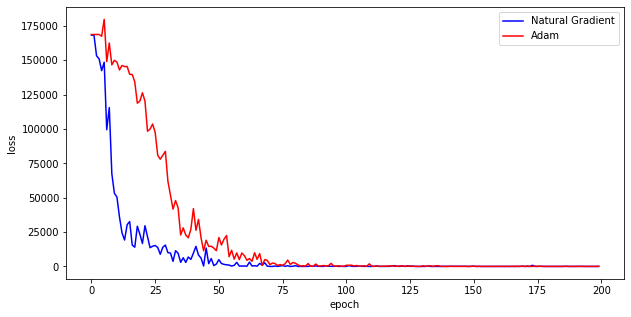
\includegraphics[width=0.4\textwidth]{images/vadam_compare.png}
\end{tabular}
\caption{The graph shows the loss versus epoch iteration of two optimization algorithm, Vadam and Adam. The blue is Vadam which uses natural gradient for update clearly converges to a loss quicker than Adam in red.}
    \label{fig:vadam_compare}
\end{figure}

We see from Figure \ref{fig:vadam_compare} that we get a quicker convergence by using natural gradient (blue) to train our model than using first-order method (red).

\section{Discussion}
Note that Vadam works very well in this case because both Vadam and I have the same assumption about the form of variation distributions and its prior. Further, Vadam is developed exactly to adapt the Adam algorithm for variational inference through natural gradient.

Although we seen how using natural gradient helps us to achieve faster convergence rate, broader application of natural gradient descant for neural network training remains restricted by the problem domain. 
Another criticism of the use of natural gradient is that, it is unclear whether the faster convergence in epoch step is justified by the slow computation of FIM. 
% Further, there are first-order heuristics which approximates the Hessian of the loss which enables Newton method for optimization. 

\section{Conclusion}

In this report we introduced the unsupervised domain adaptation problem and leveraged variational inference technique to learn a prior distribution for domain adaptation.
In addition, we shown experimentally that using natural gradient results in quicker convergence in terms of epoch step for variational inference.

In conclusion, when the situation arises, we can consider using natural gradient for model training as it yields faster model convergence.

{\small
\bibliographystyle{ieee}
\bibliography{references}
}

\end{document}
